
\documentclass[11pt]{report}
\usepackage{siunitx}
\usepackage{float}
\usepackage{graphicx}



\begin{document}
\begin{center}
	{\LARGE \textbf{Theremizer Product Design Specifications}}\\
	
	Team 18 - Bader Almatouq, Kai Brooks Jeff Roman, Andrew Forsman\\
	Version 1.0
\end{center}


	\section*{Executive Summary}
	The Theremizer is a sound control and manipulation device. It produces an audio output that sounds otherworldly and has been used in famous songs like the theme from Star Trek and the Beach Boys "Good Vibrations". It is controlled by moving your hand further or closer to an antenna to change the pitch. The Theremizer also accepts an external audio input, and if provided, will modulate this external audio input using amplitude modulation which will create interesting sounds. The Theremizer's output is then run through a classic Voltage Controlled Filter, the AS3320. This shapes the sound using resonance and by changing the cutoff to further change the sound. These are attributes that are sought after by many types of musicians, especially those interested in modular synthesis. They will incorporate the Theremizer into existing musical systems as a new sound source. Our objective is to make an affordable, interesting, musical device that can interact with other standard musical equipment. 
	\section*{Market Analysis}
	This would be primarily marketed towards analog synthesizer enthusiasts. There is a large market of modular synthesizer users that are always looking for interesting audio sources and control methods. \par There currently is nothing on the market that meets the same criteria as what the Theremizer does, as most theremins are much more expensive($>$ \$200), and the cheaper ones don't have musical filtering on the output, or any modulation possibilities within the device.
	\par We believe this device could be sold for \$120.00, as devices with a smaller feature set are being sold for \$100 currently. We are adding features (filtering, modulation) that are highly desired in the modular synthesizer community, a community that has no problem spending significant money on devices. This device should be affordable to purchase in order to compete in an otherwise cost-prohibitive marketplace.
	\section*{Requirements}
	\subsection*{Functionality}
	An antenna must modulate the frequency of an oscillator which is heterodyned with another to produce an audio output of at least one octave. The device must be capable of feeding it's output to other audio processing blocks, or a separate audio amplifier. The device must have an enclosure that is self-stable. The device should accept and modulate an external signal, then mix against the theremin output.
	\subsection*{Performance}
		To make the device useful for musicians, it will have a user controlled filter with a minimum cutoff of at least \SI{5}{\kilo\hertz}. It will have a user controlled output up to at least \SI{1}{\volt} amplitude. The output and input impedance will be compatible with industry line-level standards and will have an impedance of less than \SI{600}{\ohm} and greater than \SI{10}{\kilo\ohm} respectively. 
	\subsection*{Economic}
	The device must be affordable to produce, with a total parts cost less than \$60. All parts must be available for volume purchase, in active production, or easily substitutable by a component in current production. 
\section*{System Architecture}
	\begin{figure}[H]
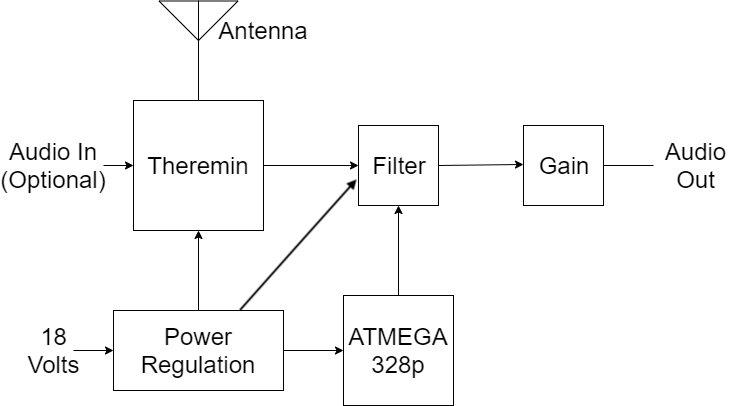
\includegraphics[width = \textwidth]{Theremizer_HighLevel_BD.png}
	\end{figure}

\section*{Design Specification}
\begin{itemize}
	\item Sensors will be the antenna in the theremin circuit, and the ADC's on the processor. Antenna will input varying capacitance based on hand distance to theremin, and ADC's will measure voltage to vary PWM from the ATMega328p to control filter cutoff, resonance and gain.
	\item Actuators will be the mixer/modulator used in the theremin circuit (currently MC1496) which will output the modulated signal, the gain stage of the filter (AS3320), and the PWM output of the ATMega328p.
	\item Processors will be the ATMega328p and the filter, the AS3320.
	\item Power will be supplied by an \SI{18}{\volt} wall transformer and regulated by two switching regulators, one for the $\pm$ \SI{15}{\volt} required for the filter and theremin and one for the \SI{5}{\volt} required for the ATMega.
	\item We will attempt to program the ATMega without using the Arduino bootloader, but may switch if neccessary. 
	\item We will use Atmel/AVR Studio to write the code and program the processor.
\end{itemize}
\end{document}
